\documentclass[hidelinks]{ctexart}

\usepackage{van-de-la-illinoise}
\usepackage[paper=b5paper,top=.3in,left=.9in,right=.9in,bottom=.3in]{geometry}
\usepackage{calc}
\pagenumbering{gobble}
\setlength{\parindent}{0pt}
\sisetup{inter-unit-product=\ensuremath{{}\cdot{}}}

\newdimen\indexlen
\def\newprobheader#1{%
\def\probindex{#1}
\setlength\indexlen{\widthof{\textbf{\probindex}}}
\hskip\dimexpr-\indexlen-1em\relax
\textbf{\probindex}\hskip1em\relax
}
\def\newprob#1{%
\newprobheader{#1}%
\def\newprob##1{%
\probsep%
\newprobheader{##1}%
}%
}
\def\probsep{\vskip1em\relax{\color{gray}\dotfill}\vskip1em\relax}

\begin{document}

\newprob{3.15}%
$\ce{^2S_{1/2}}:$ $\displaystyle g_1 = 1+\frac{j\pare{j+1} + s\pare{s+1} - l\pare{l+1}}{2j\pare{j+1}} = 2.$\\
$\ce{^2P_{1/2}}:$ $\displaystyle g_2 = 1+\frac{j\pare{j+1} + s\pare{s+1} - l\pare{l+1}}{2j\pare{j+1}} = \frac{2}{3}$.\\
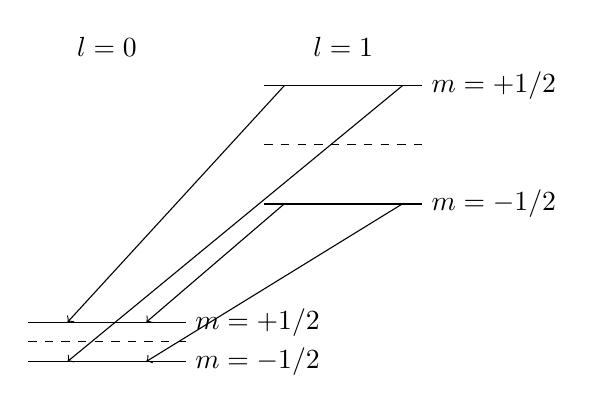
\begin{tikzpicture}
    \draw
        (0,0) -- (2,0) node[right] {$m = -1/2$}
        (0,0.5) -- (2,0.5) node[right] {$m = +1/2$}
        (3,2) -- (5,2) node[right] {$m = -1/2$}
        (3,3.5) -- (5,3.5) node[right] {$m = +1/2$}
        (1,4) node{$l=0$}
        (4,4) node{$l=1$}
    ;
    \draw[dashed]
        (0,0.25) -- (2,0.25)
        (3,2.75) -- (5,2.75)
    ;
    \draw[->] (3.25,3.5) -- (0.5,0.5);
    \draw[->] (4.75,3.5) -- (0.5,0);
    \draw[->] (3.25,2) -- (1.5,0.5);
    \draw[->] (4.75,2) -- (1.5,0);
\end{tikzpicture}\\
分裂为\underline{4条}.\\
\begin{tabular}{ccc}
    初态 & 末态 & $\displaystyle \Delta \tilde{\nu} = \+sL\cdot \pare{m_2g_2 - m_1g_1}$ \\
    $m_j=1/2$ & $m_j=1/2$ & $\displaystyle -\frac{2}{3} \times \SI{0.466}{\per\centi\meter} \times B\SI{}{\per\tesla} = \SI{0.311}{\per\centi\meter\per\tesla}$ \\[0.5em]
    $m_j=-1/2$ & $m_j=-1/2$ & $\displaystyle \frac{2}{3} \times \SI{0.466}{\per\centi\meter} \times B\SI{}{\per\tesla} = \SI{-0.311}{\per\centi\meter\per\tesla}$ \\[0.5em]
    $m_j=1/2$ & $m_j=-1/2$ & $\displaystyle \frac{4}{3} \times \SI{0.466}{\per\centi\meter} \times B\SI{}{\per\tesla} = \SI{0.621}{\per\centi\meter\per\tesla}$ \\[0.5em]
    $m_j=-1/2$ & $m_j=1/2$ & $\displaystyle -\frac{4}{3} \times \SI{0.466}{\per\centi\meter} \times B\SI{}{\per\tesla} = \SI{-0.621}{\per\centi\meter\per\tesla}$
\end{tabular}\\
$\displaystyle \Delta{\tilde{\nu}} = \frac{\Delta \lambda}{\lambda^2} = \SI{17.3}{\per\centi\meter} = \SI{0.311}{\per\centi\meter\per\tesla}\cdot B \Rightarrow B = \boxed{\SI{55.6}{\tesla}.}$
\newprob{3.16 (1)}%
共\underline{5个}能级.
\begin{tabular}[t]{cccccc}
$\ce{3S}$ & $\ce{3S_{1/2}}$ & $\ce{3P}$ & $\ce{3P_{1/2}}$ & $\ce{3D}$ & $\ce{3D_{3/2}}$ \\
 & & & $\ce{3P_{3/2}}$ & & $\ce{3D_{5/2}}$
\end{tabular}
\par
\newprobheader{(2)}%
分裂为\underline{14个}能级.\\[-1.5\baselineskip]
\begin{textblock}{3}(7,9)
    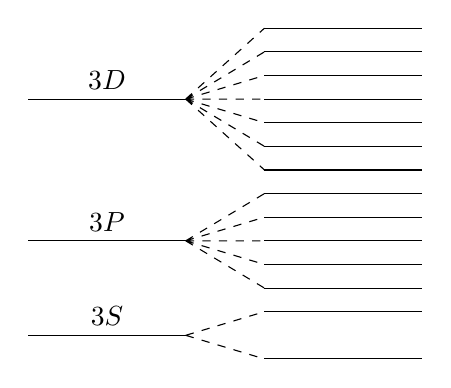
\begin{tikzpicture}[yscale=0.3]
        \draw
            (0,0) -- (2,0)
            (0,4) -- (2,4)
            (0,10) -- (2,10)
            (1,0) node[above] {$\ce{3S}$}
            (1,4) node[above] {$\ce{3P}$}
            (1,10) node[above] {$\ce{3D}$}
        ;
        \draw
            (3,-1) -- (5,-1)
            (3,1) -- (5,1)
            %
            (3,2) -- (5,2)
            (3,3) -- (5,3)
            (3,4) -- (5,4)
            (3,5) -- (5,5)
            (3,6) -- (5,6)
            %
            (3,7) -- (5,7)
            (3,8) -- (5,8)
            (3,9) -- (5,9)
            (3,10) -- (5,10)
            (3,11) -- (5,11)
            (3,12) -- (5,12)
            (3,13) -- (5,13)
        ;
        \draw[dashed]
            (2,0) -- (3,-1)
            (2,0) -- (3,1)
            %
            (2,4) -- (3,2)
            (2,4) -- (3,3)
            (2,4) -- (3,4)
            (2,4) -- (3,5)
            (2,4) -- (3,6)
            %
            (2,10) -- (3,7)
            (2,10) -- (3,8)
            (2,10) -- (3,9)
            (2,10) -- (3,10)
            (2,10) -- (3,11)
            (2,10) -- (3,12)
            (2,10) -- (3,13)
        ;
    \end{tikzpicture}
\end{textblock}%
\begin{longtable}[l]{cccc}
    轨道 & $m_l$ & $m_s$ & $m_l + 2m_s$ \\
    $\ce{3D}$ & $2$ & $+1/2$ & $3$ \\
    & $1$ & $+1/2$ & $2$ \\
    & $2$ & $-1/2$ & \+:r2{$1$} \\
    & $0$ & $+1/2$ & \\
    & $1$ & $-1/2$ & \+:r2{$0$} \\
    & $-1$ & $+1/2$ & \\
    & $-2$ & $+1/2$ & \+:r2{$-1$} \\
    & $0$ & $-1/2$ & \\
    & $-1$ & $-1/2$ & $-2$ \\
    & $-2$ & $-1/2$ & $-3$ \\
    $\ce{3P}$ & $1$ & $+1/2$ & $2$ \\
    & $0$& $+1/2$ & $1$ \\
    & $1$& $-1/2$ & \+:r2{$0$} \\
    & $-1$ & $+1/2$ & \\
    & $0$ & $-1/2$ & $-1$ \\
    & $-1$ & $-1/2$ & $-2$ \\
    $\ce{3S}$ & $0$ & $+1/2$ & $1$ \\
    & $0$ & $-1/2$ & $-1$
\end{longtable}
\newprob{3.17}%
基态$\ce{^2S_{1/2}}$, $\displaystyle g = 1 + \frac{j\pare{j+1} + s\pare{s+1} - l\pare{l+1}}{2j\pare{j+1}} = 2$.\\
$\displaystyle \Delta E = g \Delta m \mu\+_B_ B = 2\times 1 \times \SI{5.79e-5}{\eV} = \boxed{\SI{1.16e-4}{\eV}.}$\\
$\nu = \frac{\Delta E}{h} = \boxed{\SI{2.8e10}{\hertz}.}$
\newprob{3.18}%
$I = 1/2$, $J = 1/2$, $F = \curb{0, 1}$. \\
$\displaystyle \Delta E = \frac{a}{2}\brac{F\pare{F+1} - J\pare{J+1} - I\pare{I+1}} = \curb{\frac{a}{4},-\frac{3a}{4}}$.\\
$\displaystyle \delta E = a = h \nu = \boxed{\SI{5.87e-6}{\eV}.}$
\newprob{3.19}%
$\displaystyle \Delta E = h\nu = \SI{8.27e-5}{\eV} = g \mu\+_B_ B \Rightarrow g = \boxed{\frac{4}{5}} = 1 + \frac{j\pare{j+1} + l\pare{l+1} - s\pare{s+1}}{2j\pare{j+1}}$,\\
$s=1/2$, $j = l\pm 1/2 \Rightarrow l = 2, j = 3/2 \Rightarrow $处于\underline{$\ce{^2D_{3/2}}$态}.

\end{document}
